% Based on code by Stefan Kottwitz
\documentclass[border = 10pt]{standalone}
\usepackage{tikz}
\usetikzlibrary{circuits.ee.IEC}
\begin{document}
\begin{tikzpicture}[
    circuit ee IEC,
    x = 3cm, y = 2cm,
    every info/.style = {font = \scriptsize},
    set diode graphic = var diode IEC graphic,
    set make contact graphic = var make contact IEC graphic,
  ]
  \foreach \i in {2,...,3} {
    \node [contact] (upper contact \i) at (\i,1) {};
    \node [contact] (lower contact \i) at (\i+2, 1) {};
  }

  \draw (upper contact 2) to [make contact = {near start, info = $x_1$ x1 x$_1$}]
        (upper contact 3);
  \draw (lower contact 2) to [make contact = {near end, info = $x_2$ x2 x$_2$}]
  		(lower contact 3);
\end{tikzpicture}
text between pictures\\
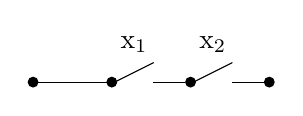
\begin{tikzpicture}
[circuit ee IEC]
\foreach \i in {1,...,4}{
	\node [contact] (contact \i) at (\i, 0) {};
}
\draw (contact 1) to (contact 2);
\draw (contact 2) to [make contact = {near start, info = x$_1$}]
 (contact 3);
\draw (contact 3) to [make contact = {near start, info = x$_2$}]
 (contact 4);
\end{tikzpicture}
text\\
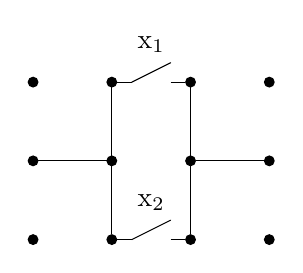
\begin{tikzpicture}
[circuit ee IEC]
\foreach \i in {1,...,4}{
	\node [contact] (up\i) at (\i, 2) {};
	\node [contact] (mid\i) at (\i, 1) {};
	\node [contact] (down\i) at (\i, 0) {};
}
\draw (mid1) to (mid2);
\draw (mid2) to (up2);
\draw (mid2) to (down2);

\draw (up2) to [make contact = {midway, info = x$_1$}] (up3);
\draw (down2) to [make contact = {midway, info = x$_2$}] (down3);

\draw (up3) to (mid3);
\draw (down3) to (mid3);
\draw (mid3) to (mid4);
\end{tikzpicture}
\end{document}